%-------------------------------------------------------------------------------
% Preamble
%-------------------------------------------------------------------------------

\documentclass[a4paper, 12pt]{article}
\usepackage[osf]{mathpazo} % palatino
%\usepackage[round]{natbib} % author-year citations
\usepackage[superscript,biblabel]{cite} % for superscript citations
\usepackage{graphicx}
\usepackage{subcaption}
\usepackage{parskip} 
\usepackage{amsmath}
\usepackage{longtable}
\usepackage{pdflscape}
\usepackage{array}
\usepackage{float}

\pagenumbering{arabic}  
\linespread{1.3}

% figure numbering override
\renewcommand*{\thefigure}{A\arabic{figure}} % make Fig A1 not Fig 1
\renewcommand*{\thetable}{A\arabic{table}} % make Table A1 not Table 1

%-------------------------------------------------------------------------------
% Title page information
%-------------------------------------------------------------------------------

\title{Supplementary Information from: \textit{Sex biases in bird and mammal natural history collections}}

\author{Natalie Cooper, 
  Alexander L. Bond,
  Kristofer M. Helgen,\\
  Roberto Portela Miguez and
  Louise Tomsett}

\date{}

% End of preamble

\begin{document}

\maketitle

\parindent = 1.5em
\addtolength{\parskip}{.3em}

%-------------------------------------------------------------------------------
% Figures
%-------------------------------------------------------------------------------

\section*{Supplementary Figures} 

% figure A1
\begin{figure}[H]
 \centering
  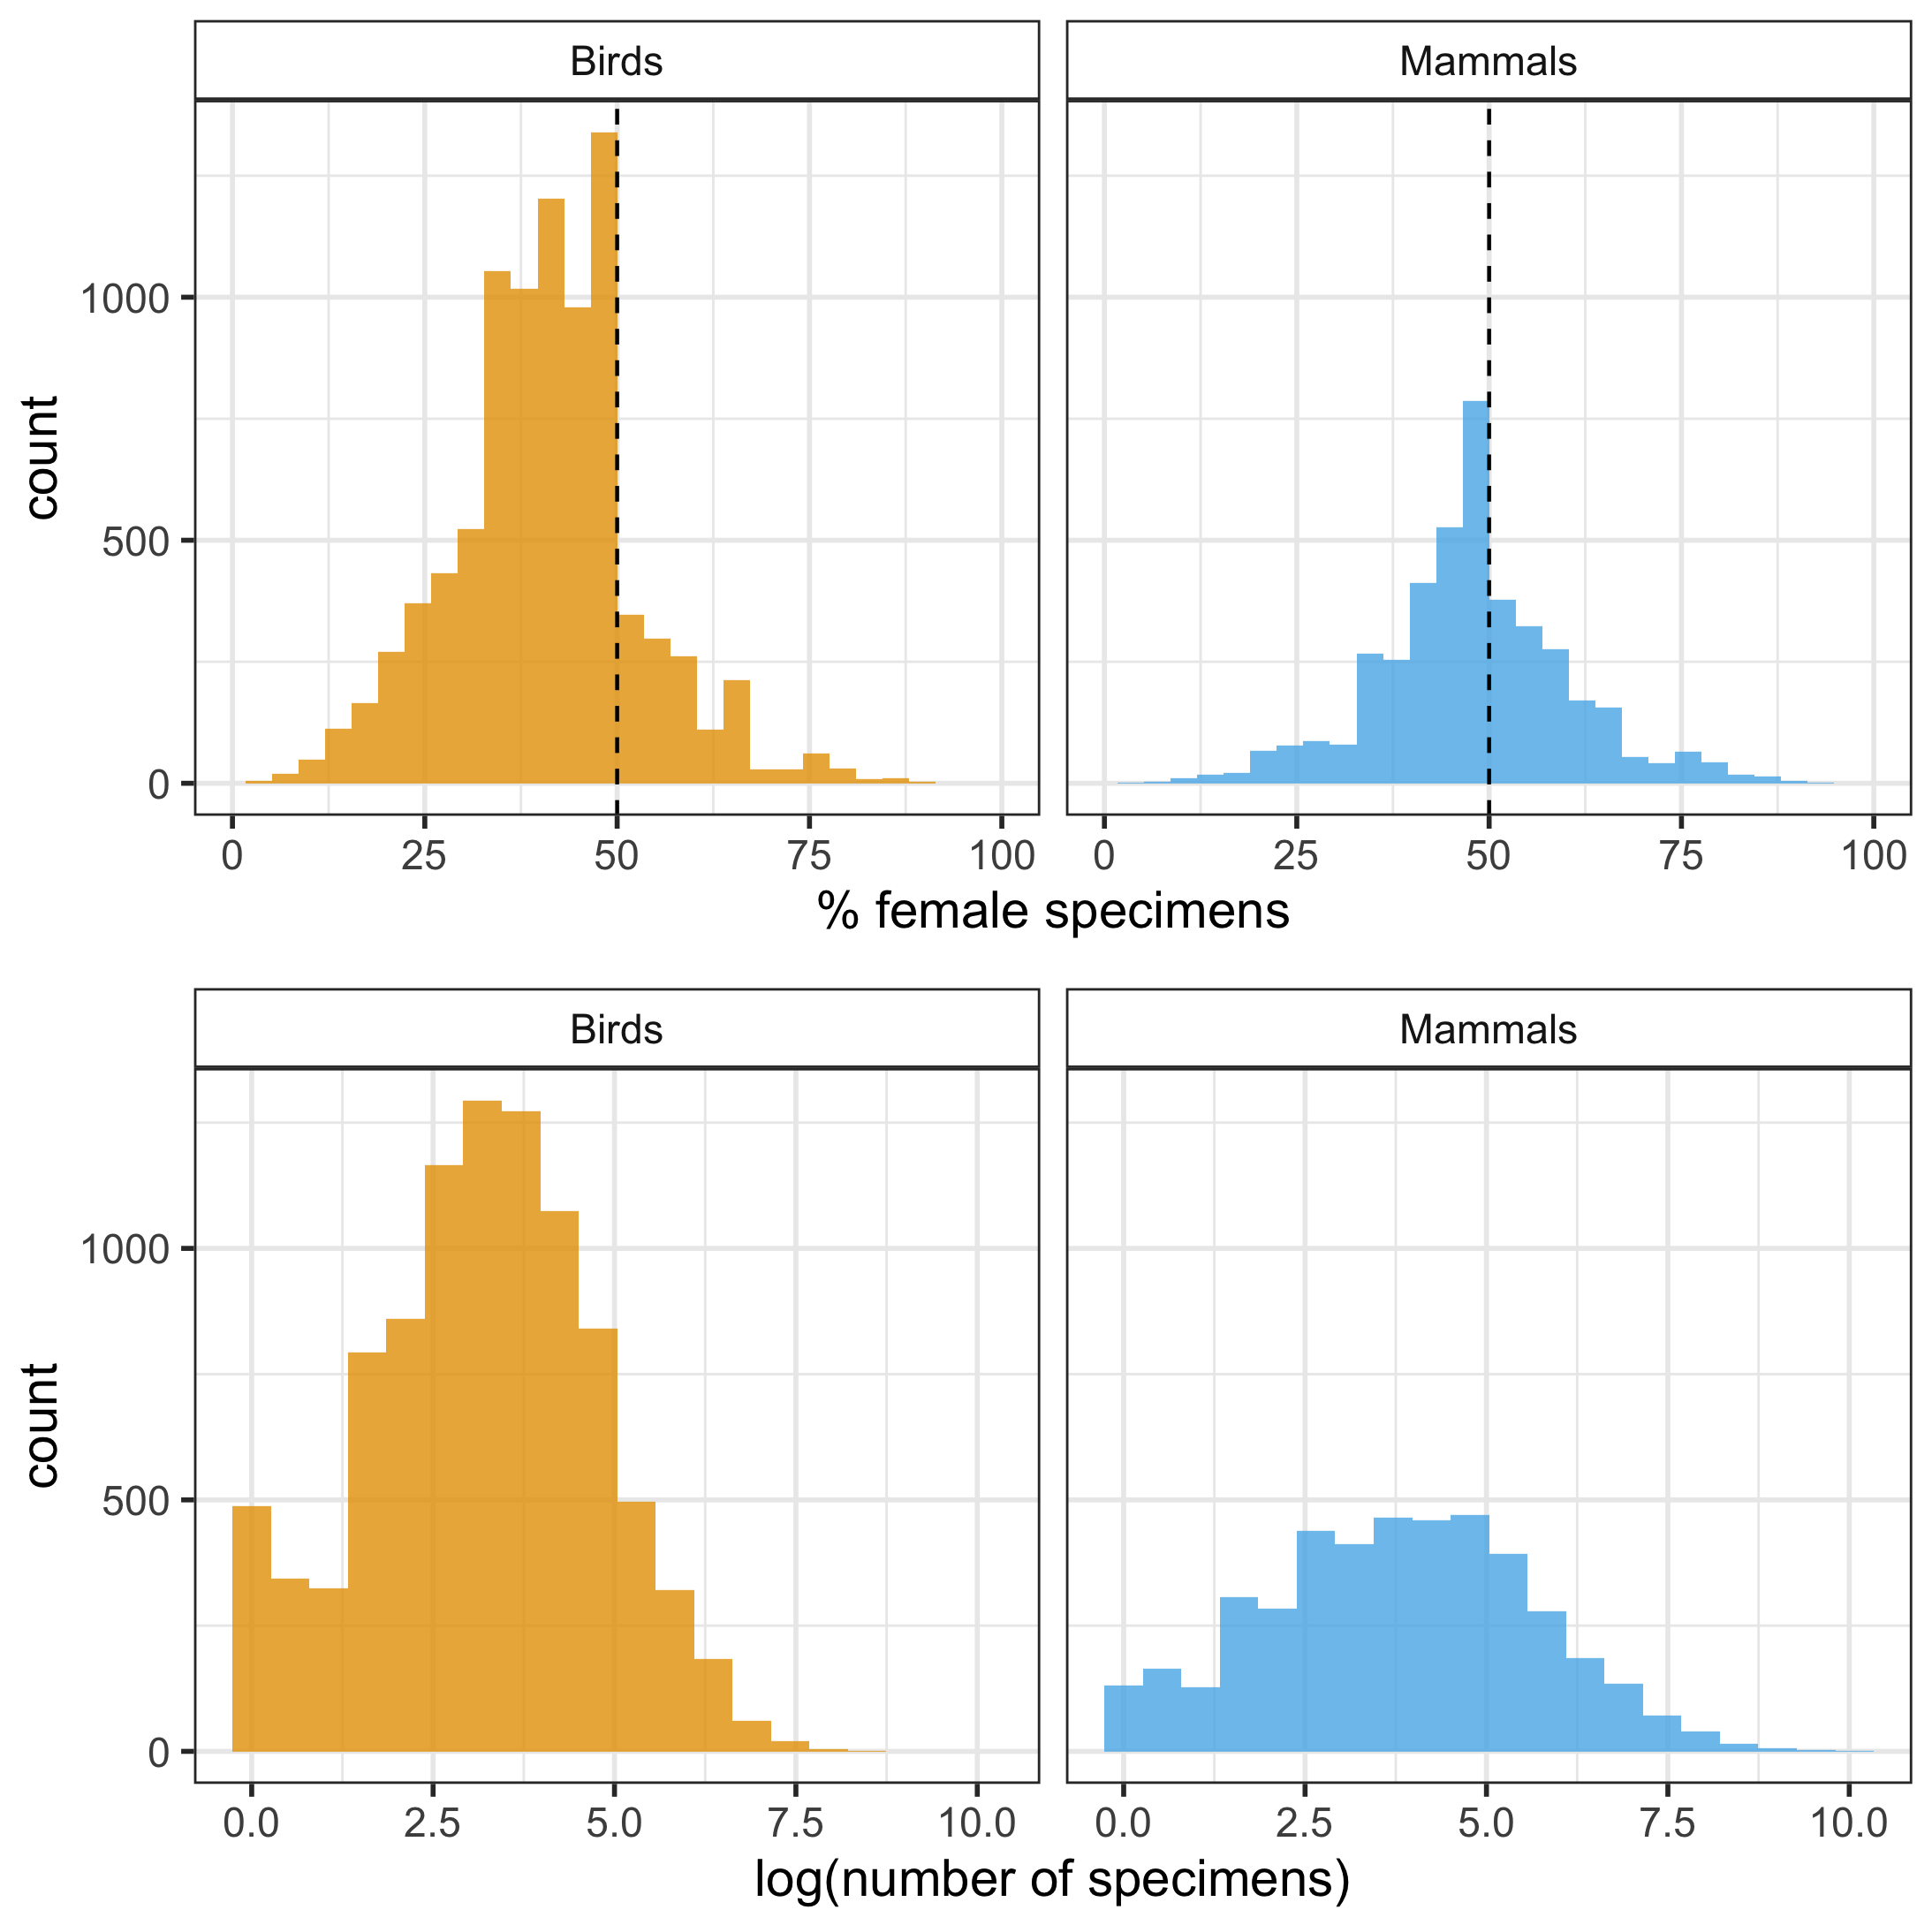
\includegraphics[width = \linewidth]{figures/histogram-specimen-counts.png}
  \caption{Histograms showing the distribution of percentage female specimens and log number of specimens for each species across birds and mammals.}
  \label{fig-histograms}
\end{figure}

% figure A2
\begin{figure}[H]
 \centering
  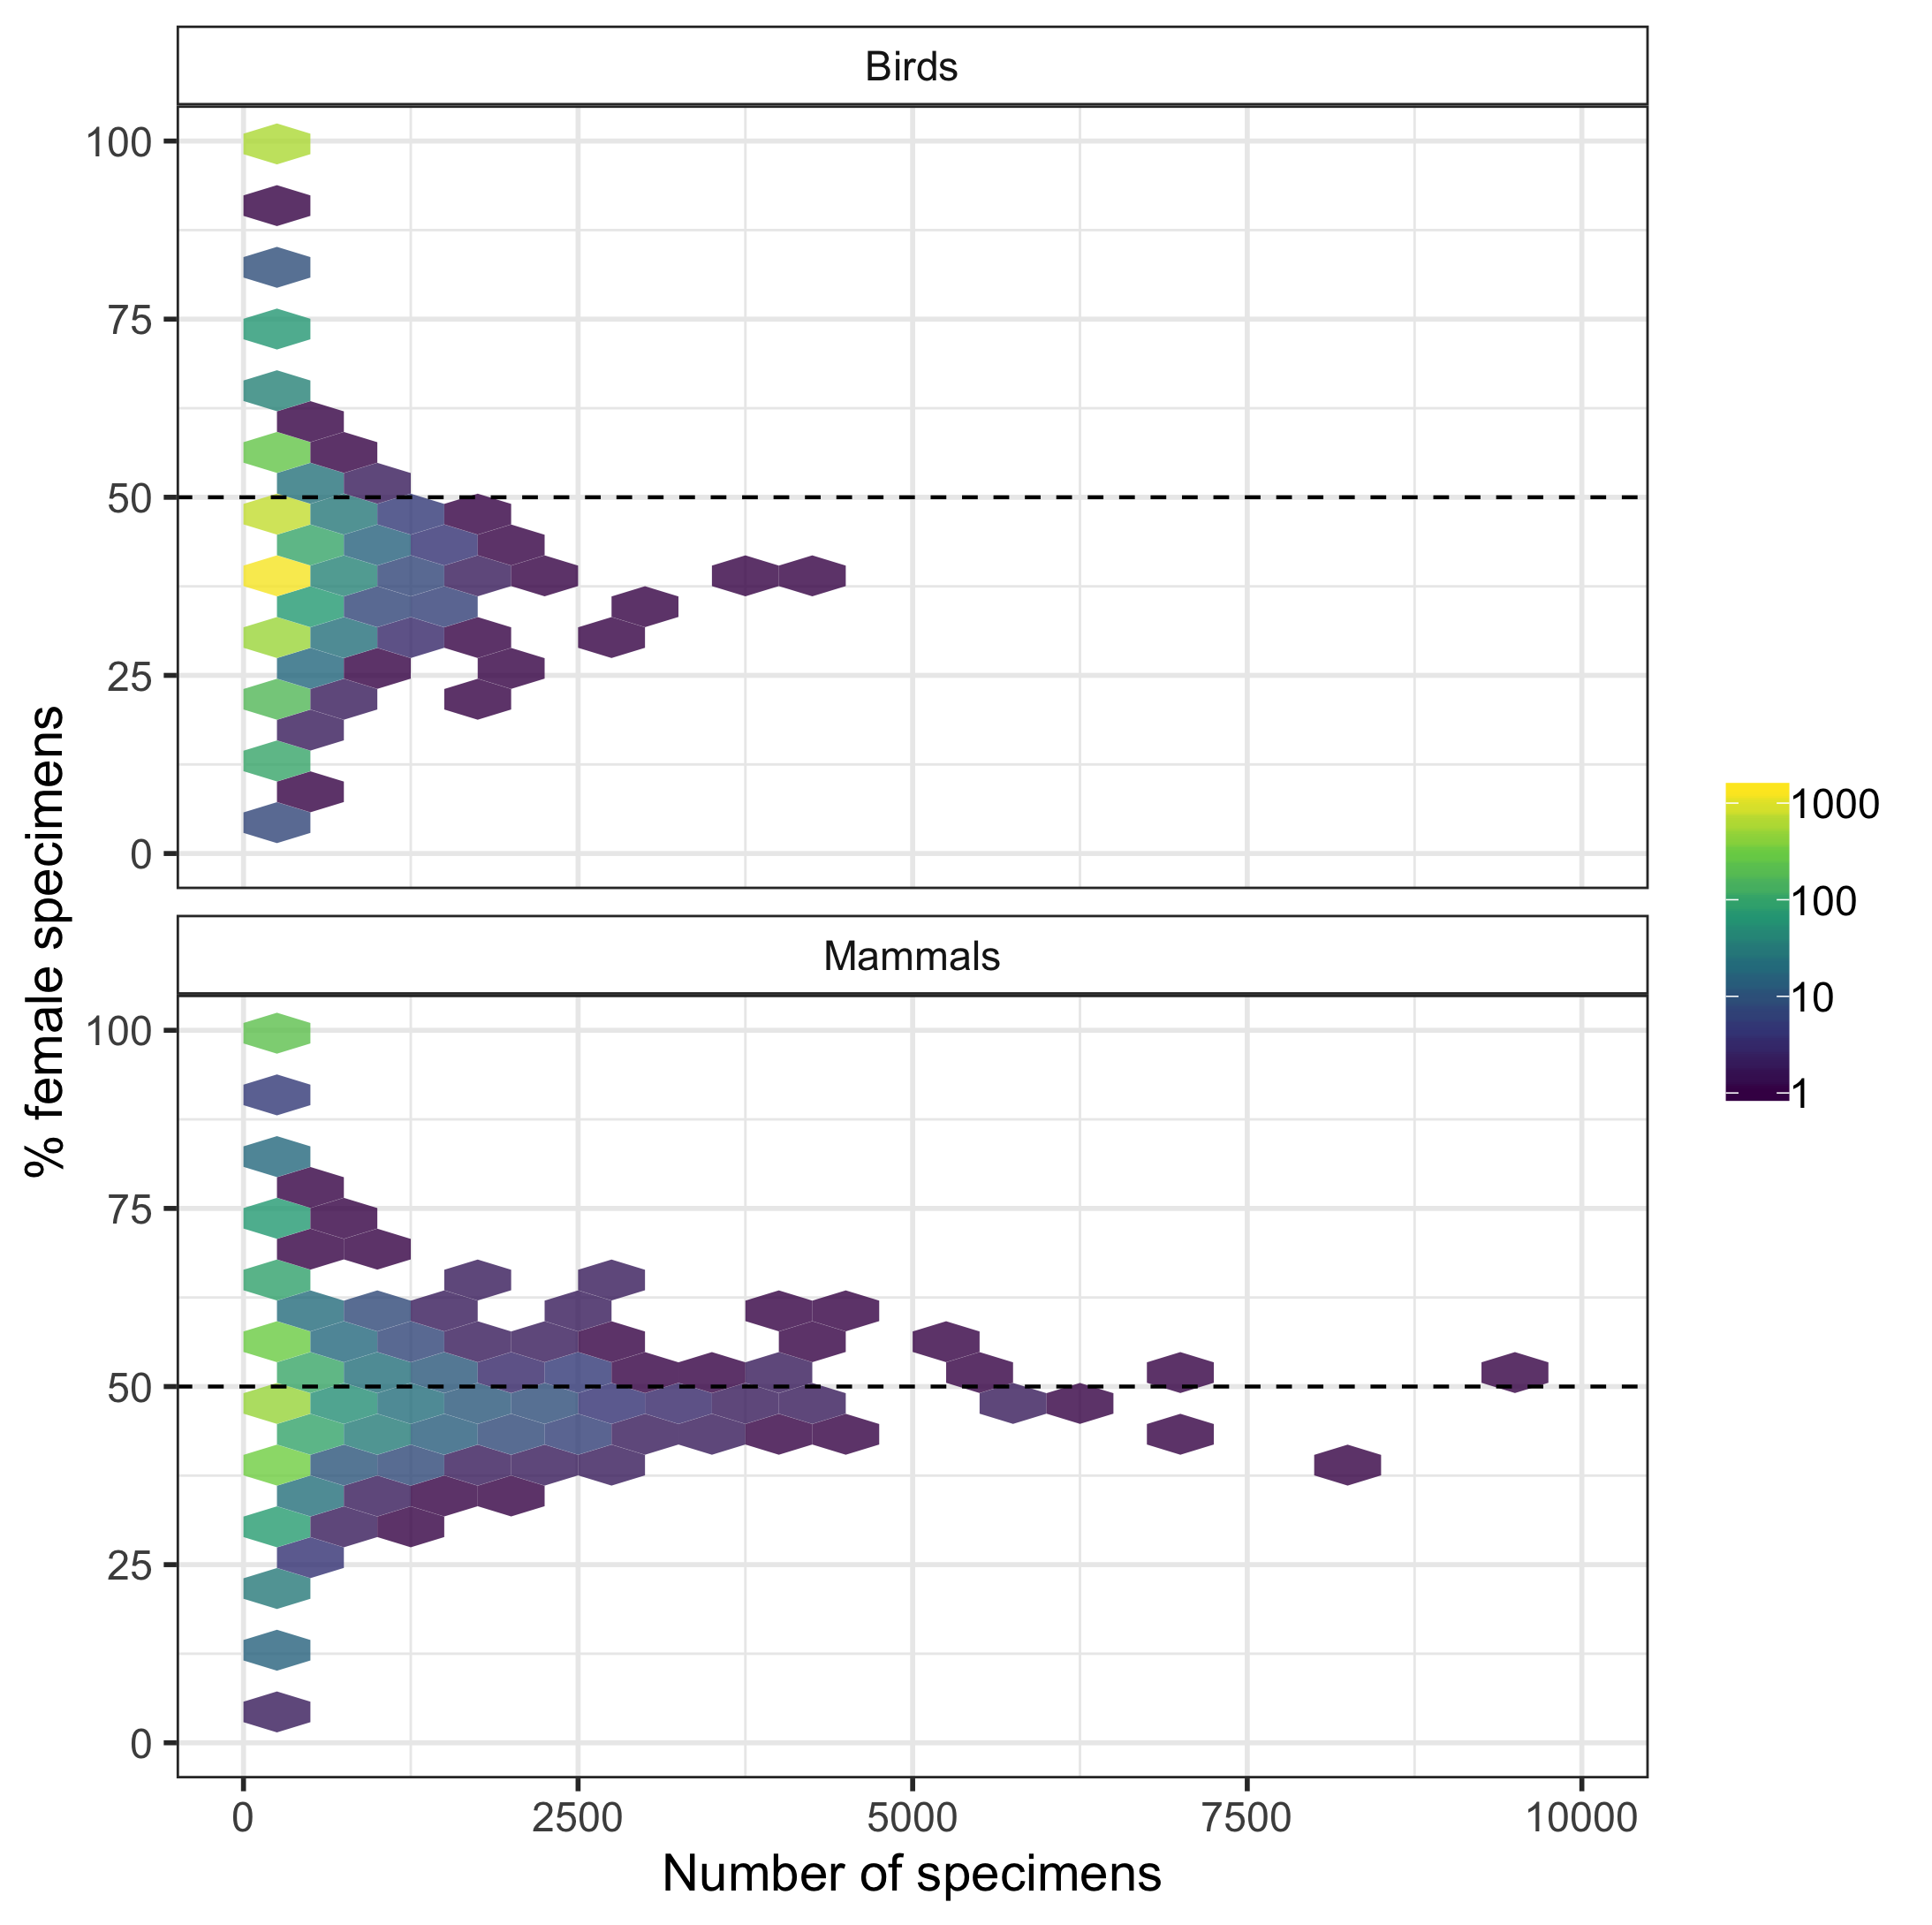
\includegraphics[width = \linewidth]{figures/specimens-numbers-all.png}
  \caption{Relationship between the percentage female specimens in each species and the number of specimens for each species. 
  Hex bins are used rather than points to make the plot easier to read.}
  \label{fig-hex}
\end{figure}

% figure A3
\begin{figure}[H]
 \centering
  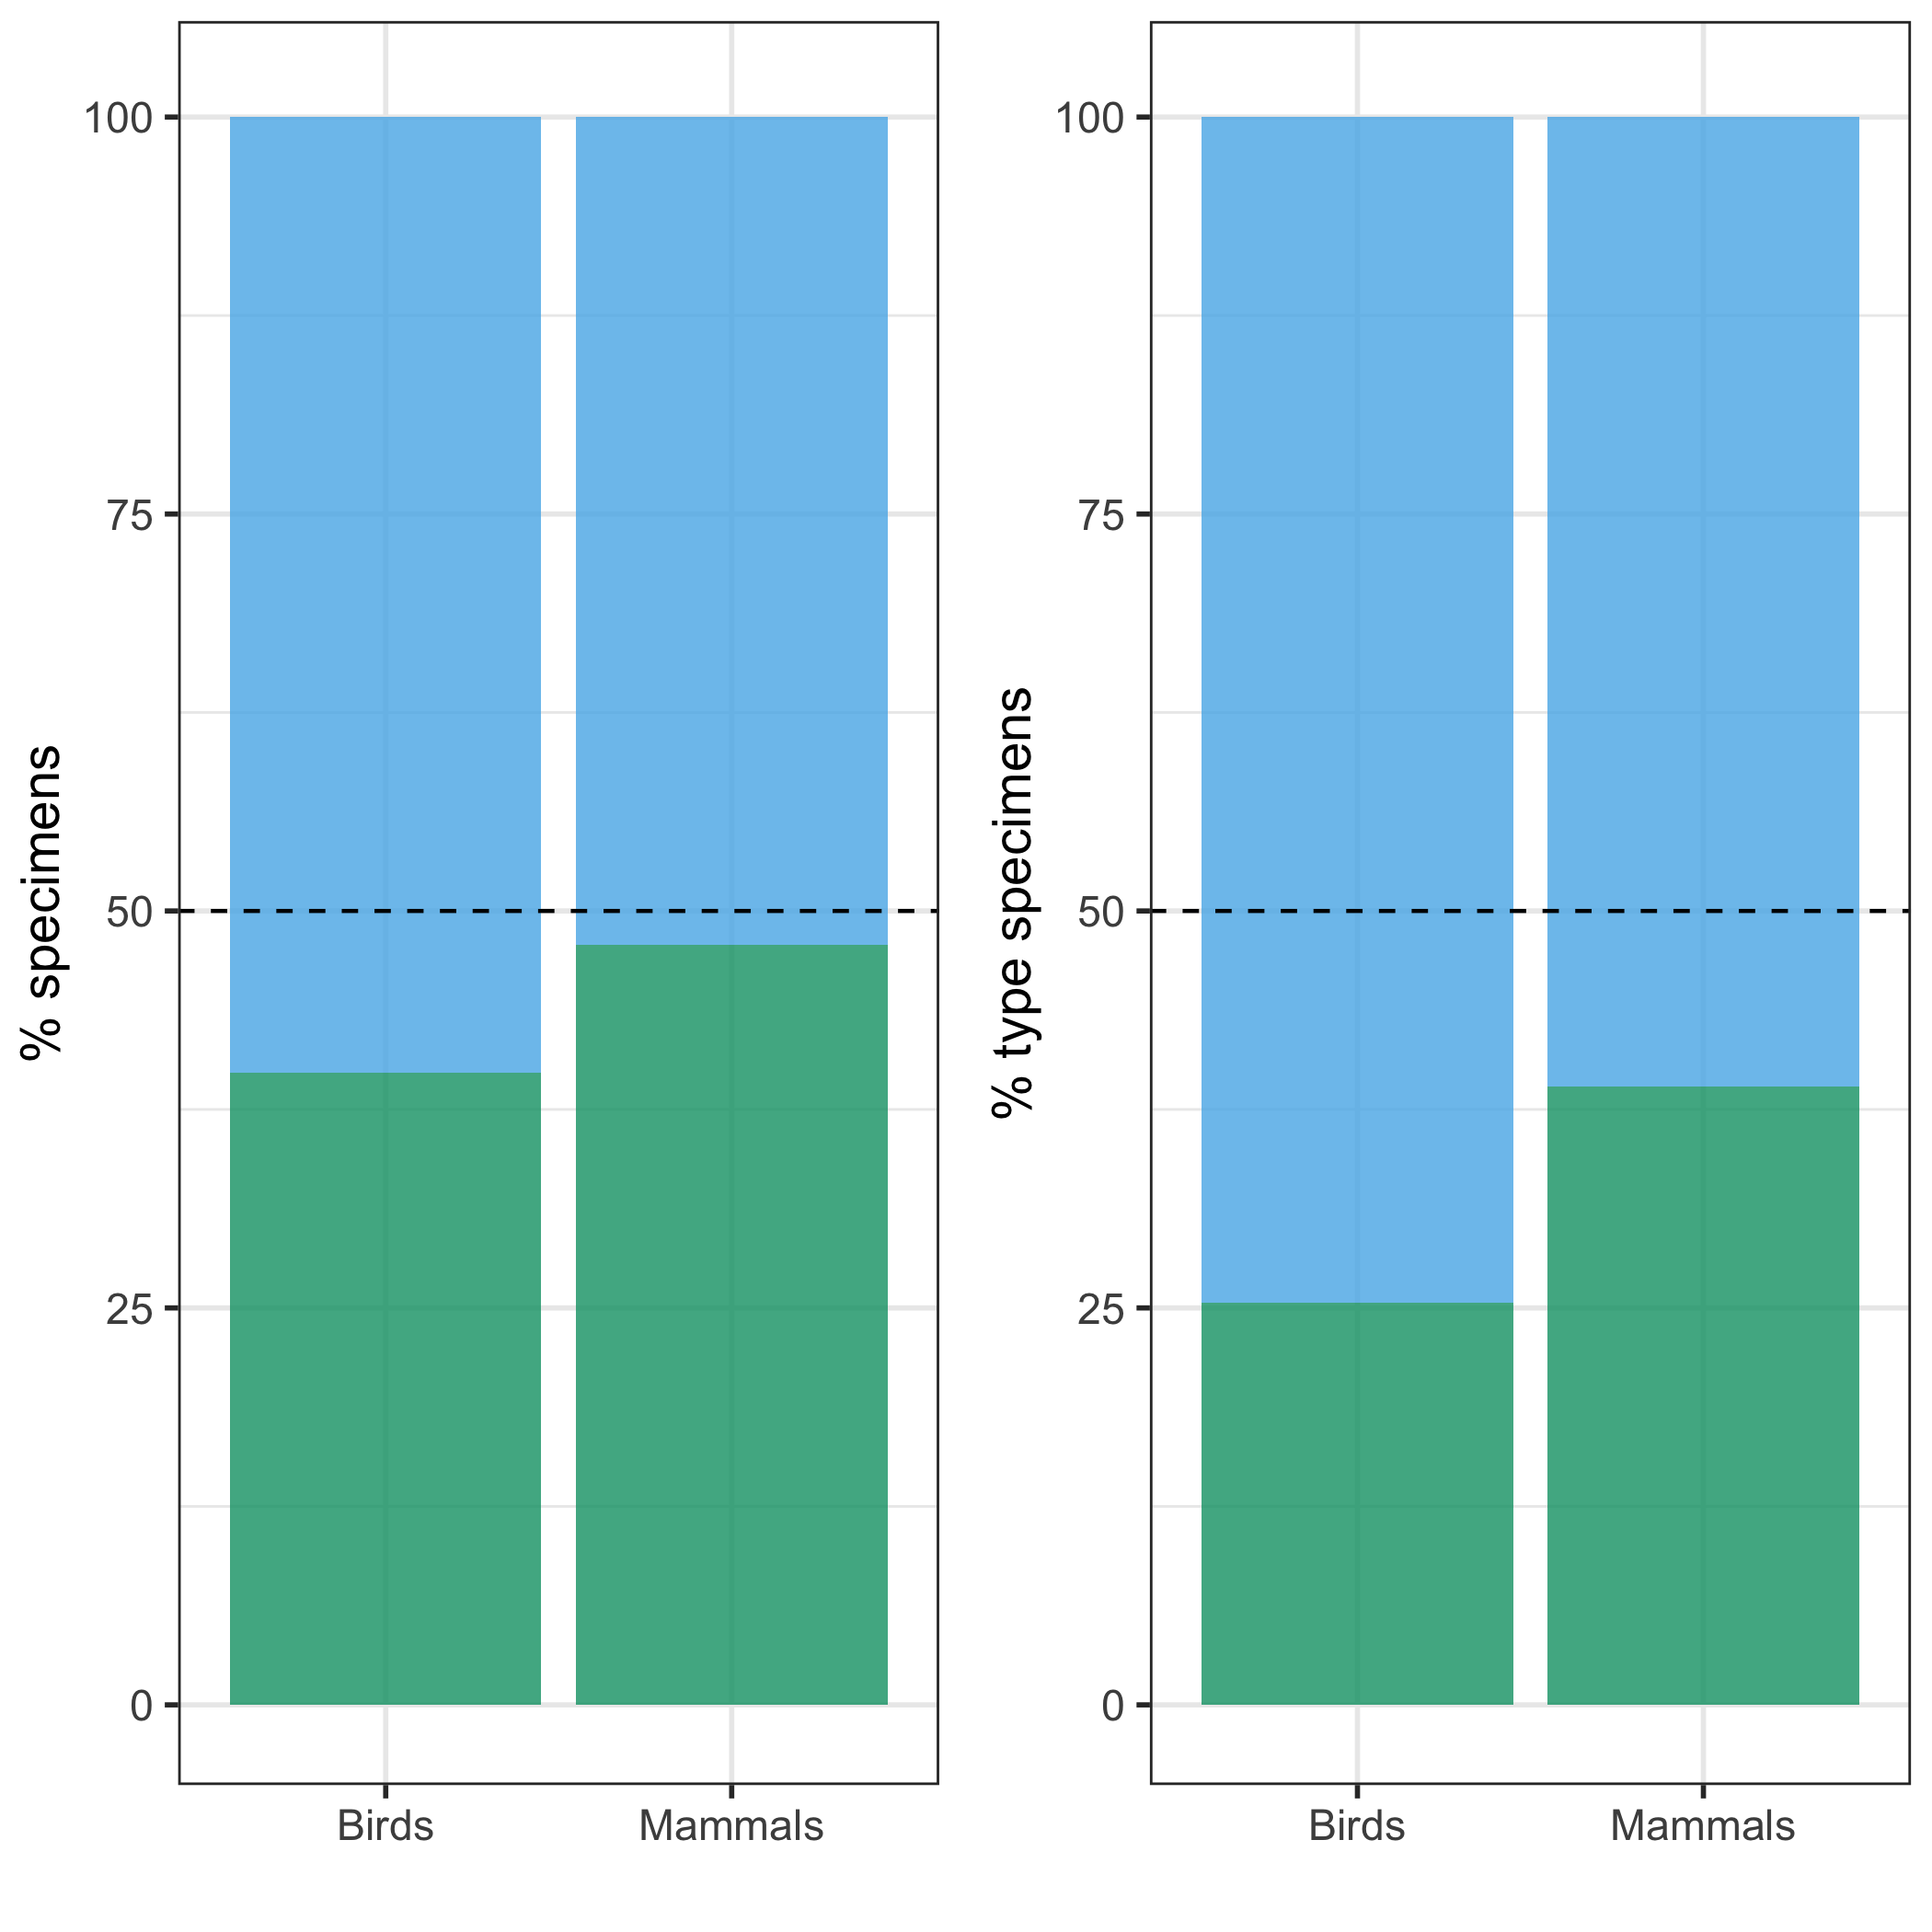
\includegraphics[width = \linewidth]{figures/types-all.png}
  \caption{Percentages of female (green) and male (blue) specimens in bird and mammal collections for all specimens (left hand panel) and for name-bearing type specimens only (right hand panel). 
  The dashed line represents 50\% female specimens.}
  \label{fig-types}
\end{figure}

% figure A4
\begin{figure}
 \centering
  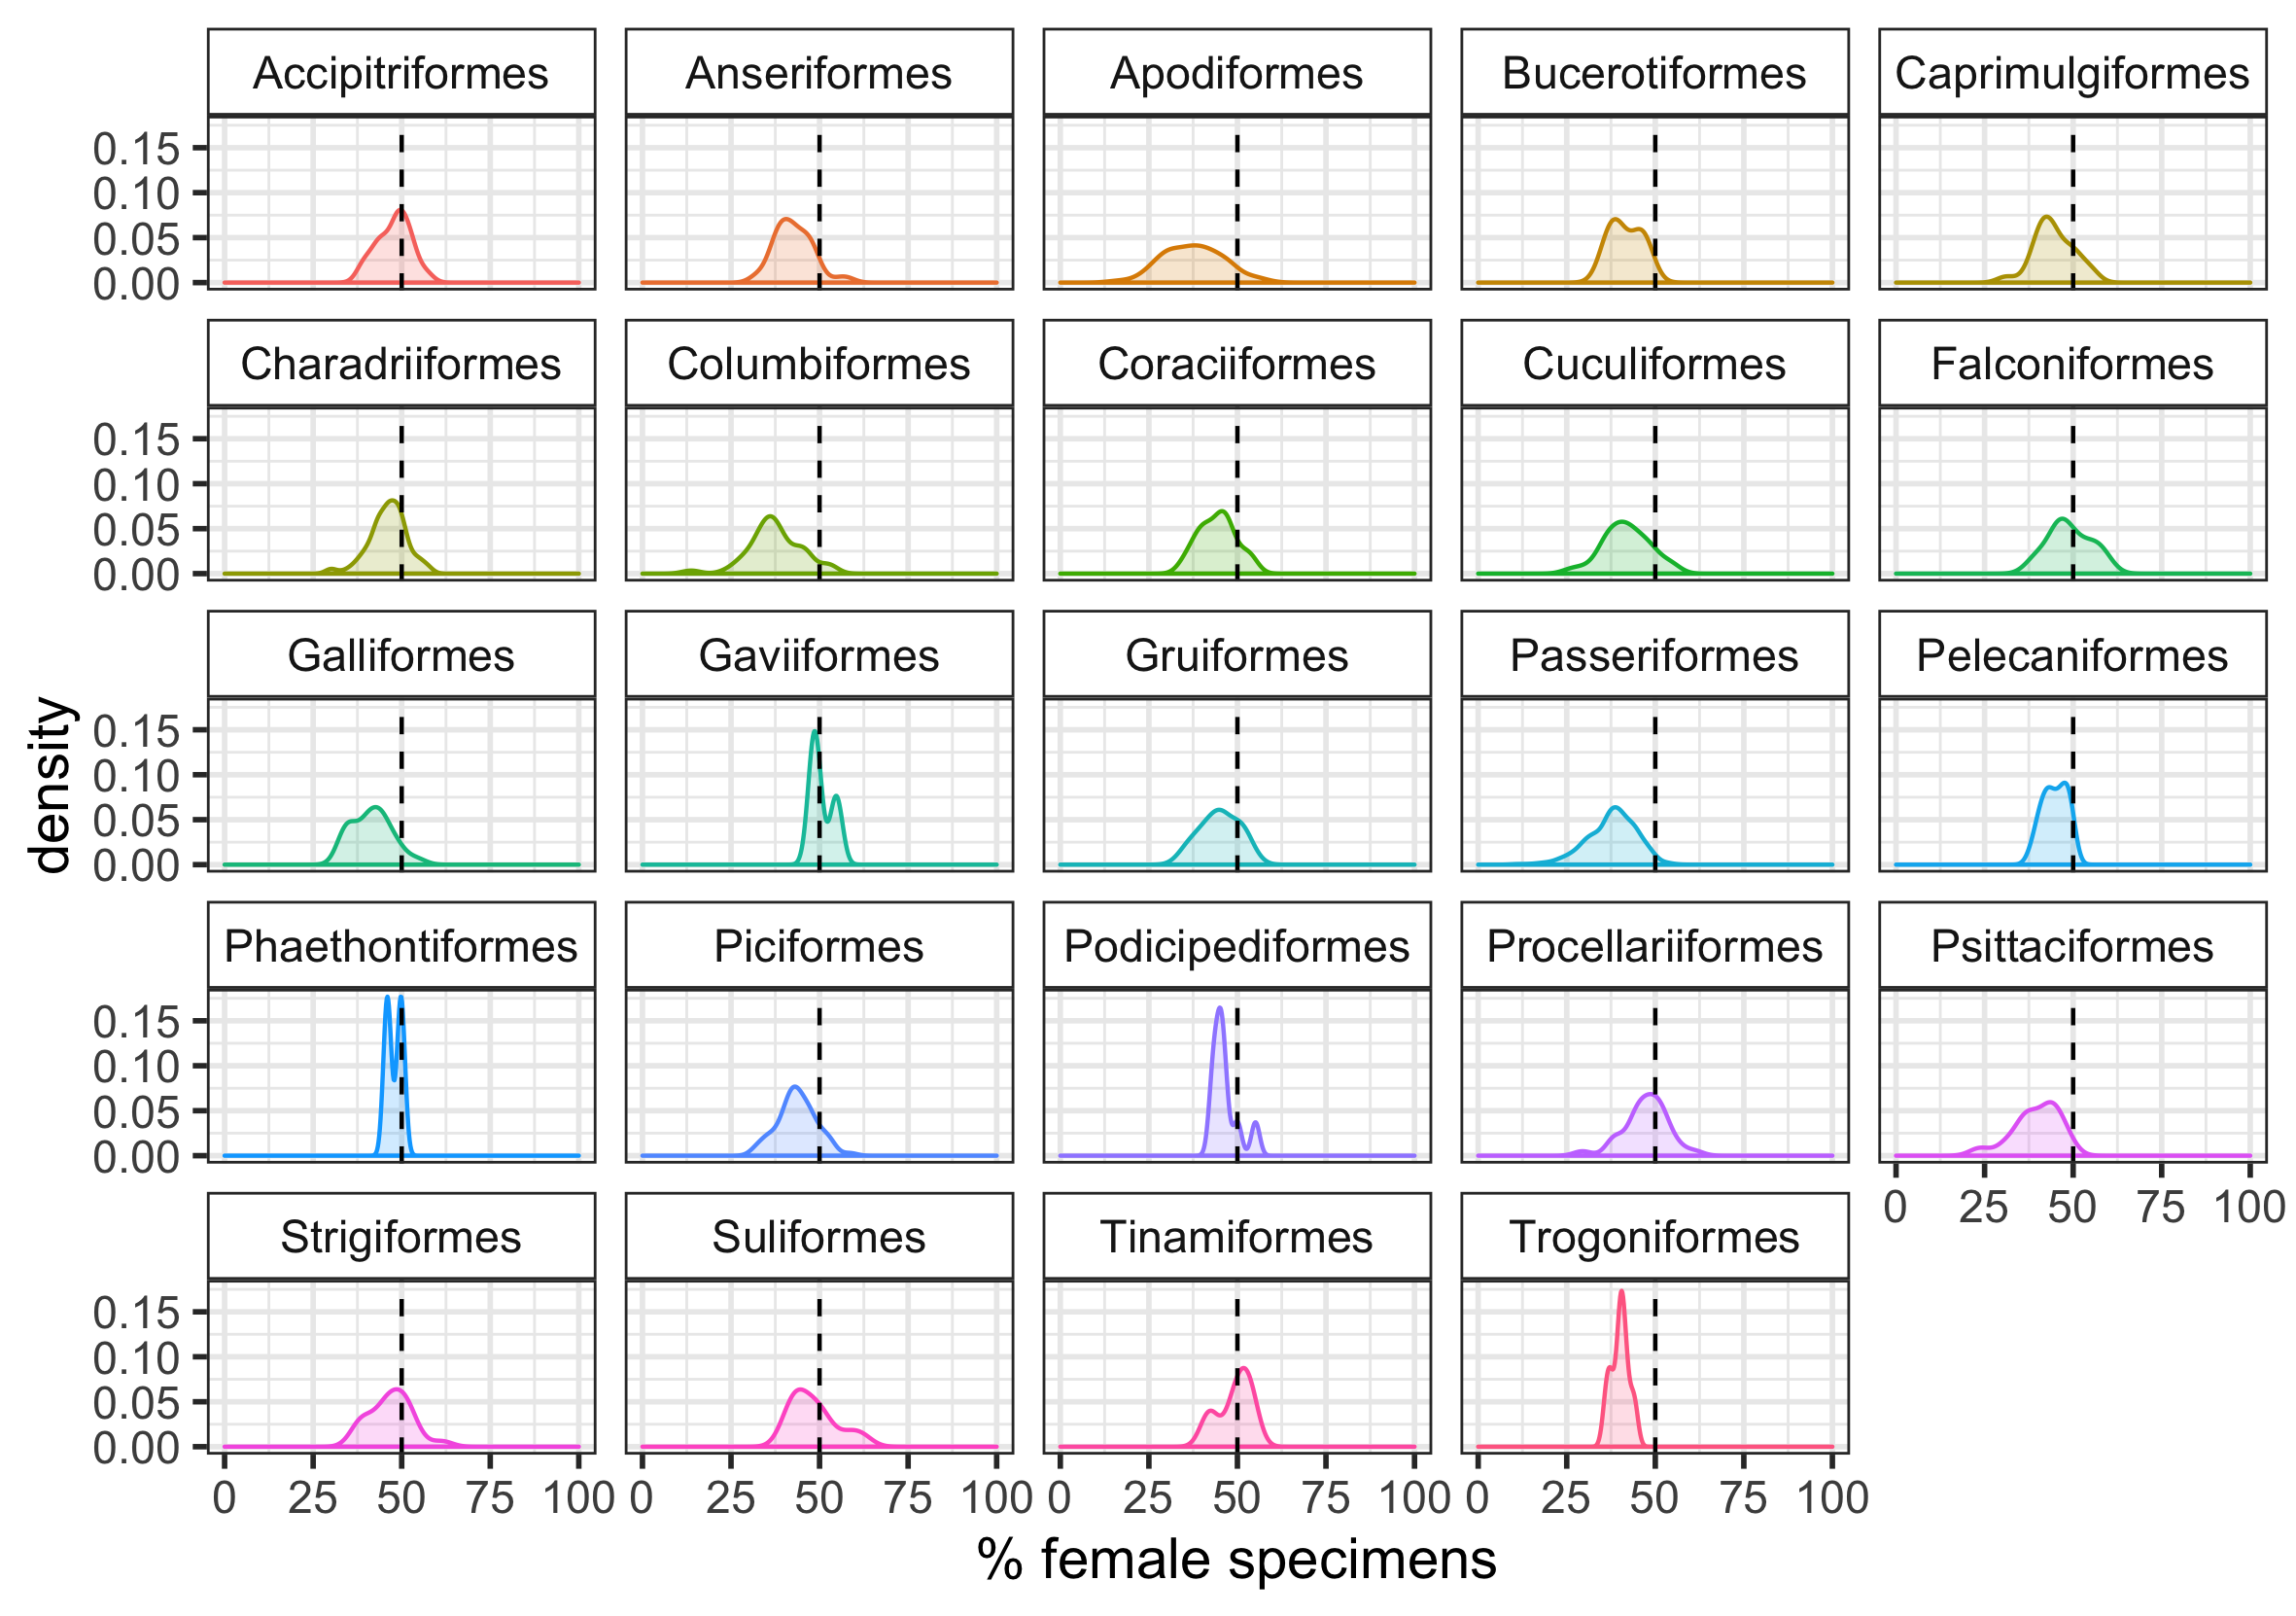
\includegraphics[width = \linewidth]{figures/orders-density-birds-all.png}
  \caption{Kernel density plots showing the \% female specimens in each species across orders of birds with at least three species in the dataset. 
  Only species with at least 100 specimens are included. 
  The dashed line represents 50\% female specimens.}
  \label{fig-bird-orders}
\end{figure}

% figure A5
\begin{figure}
 \centering
  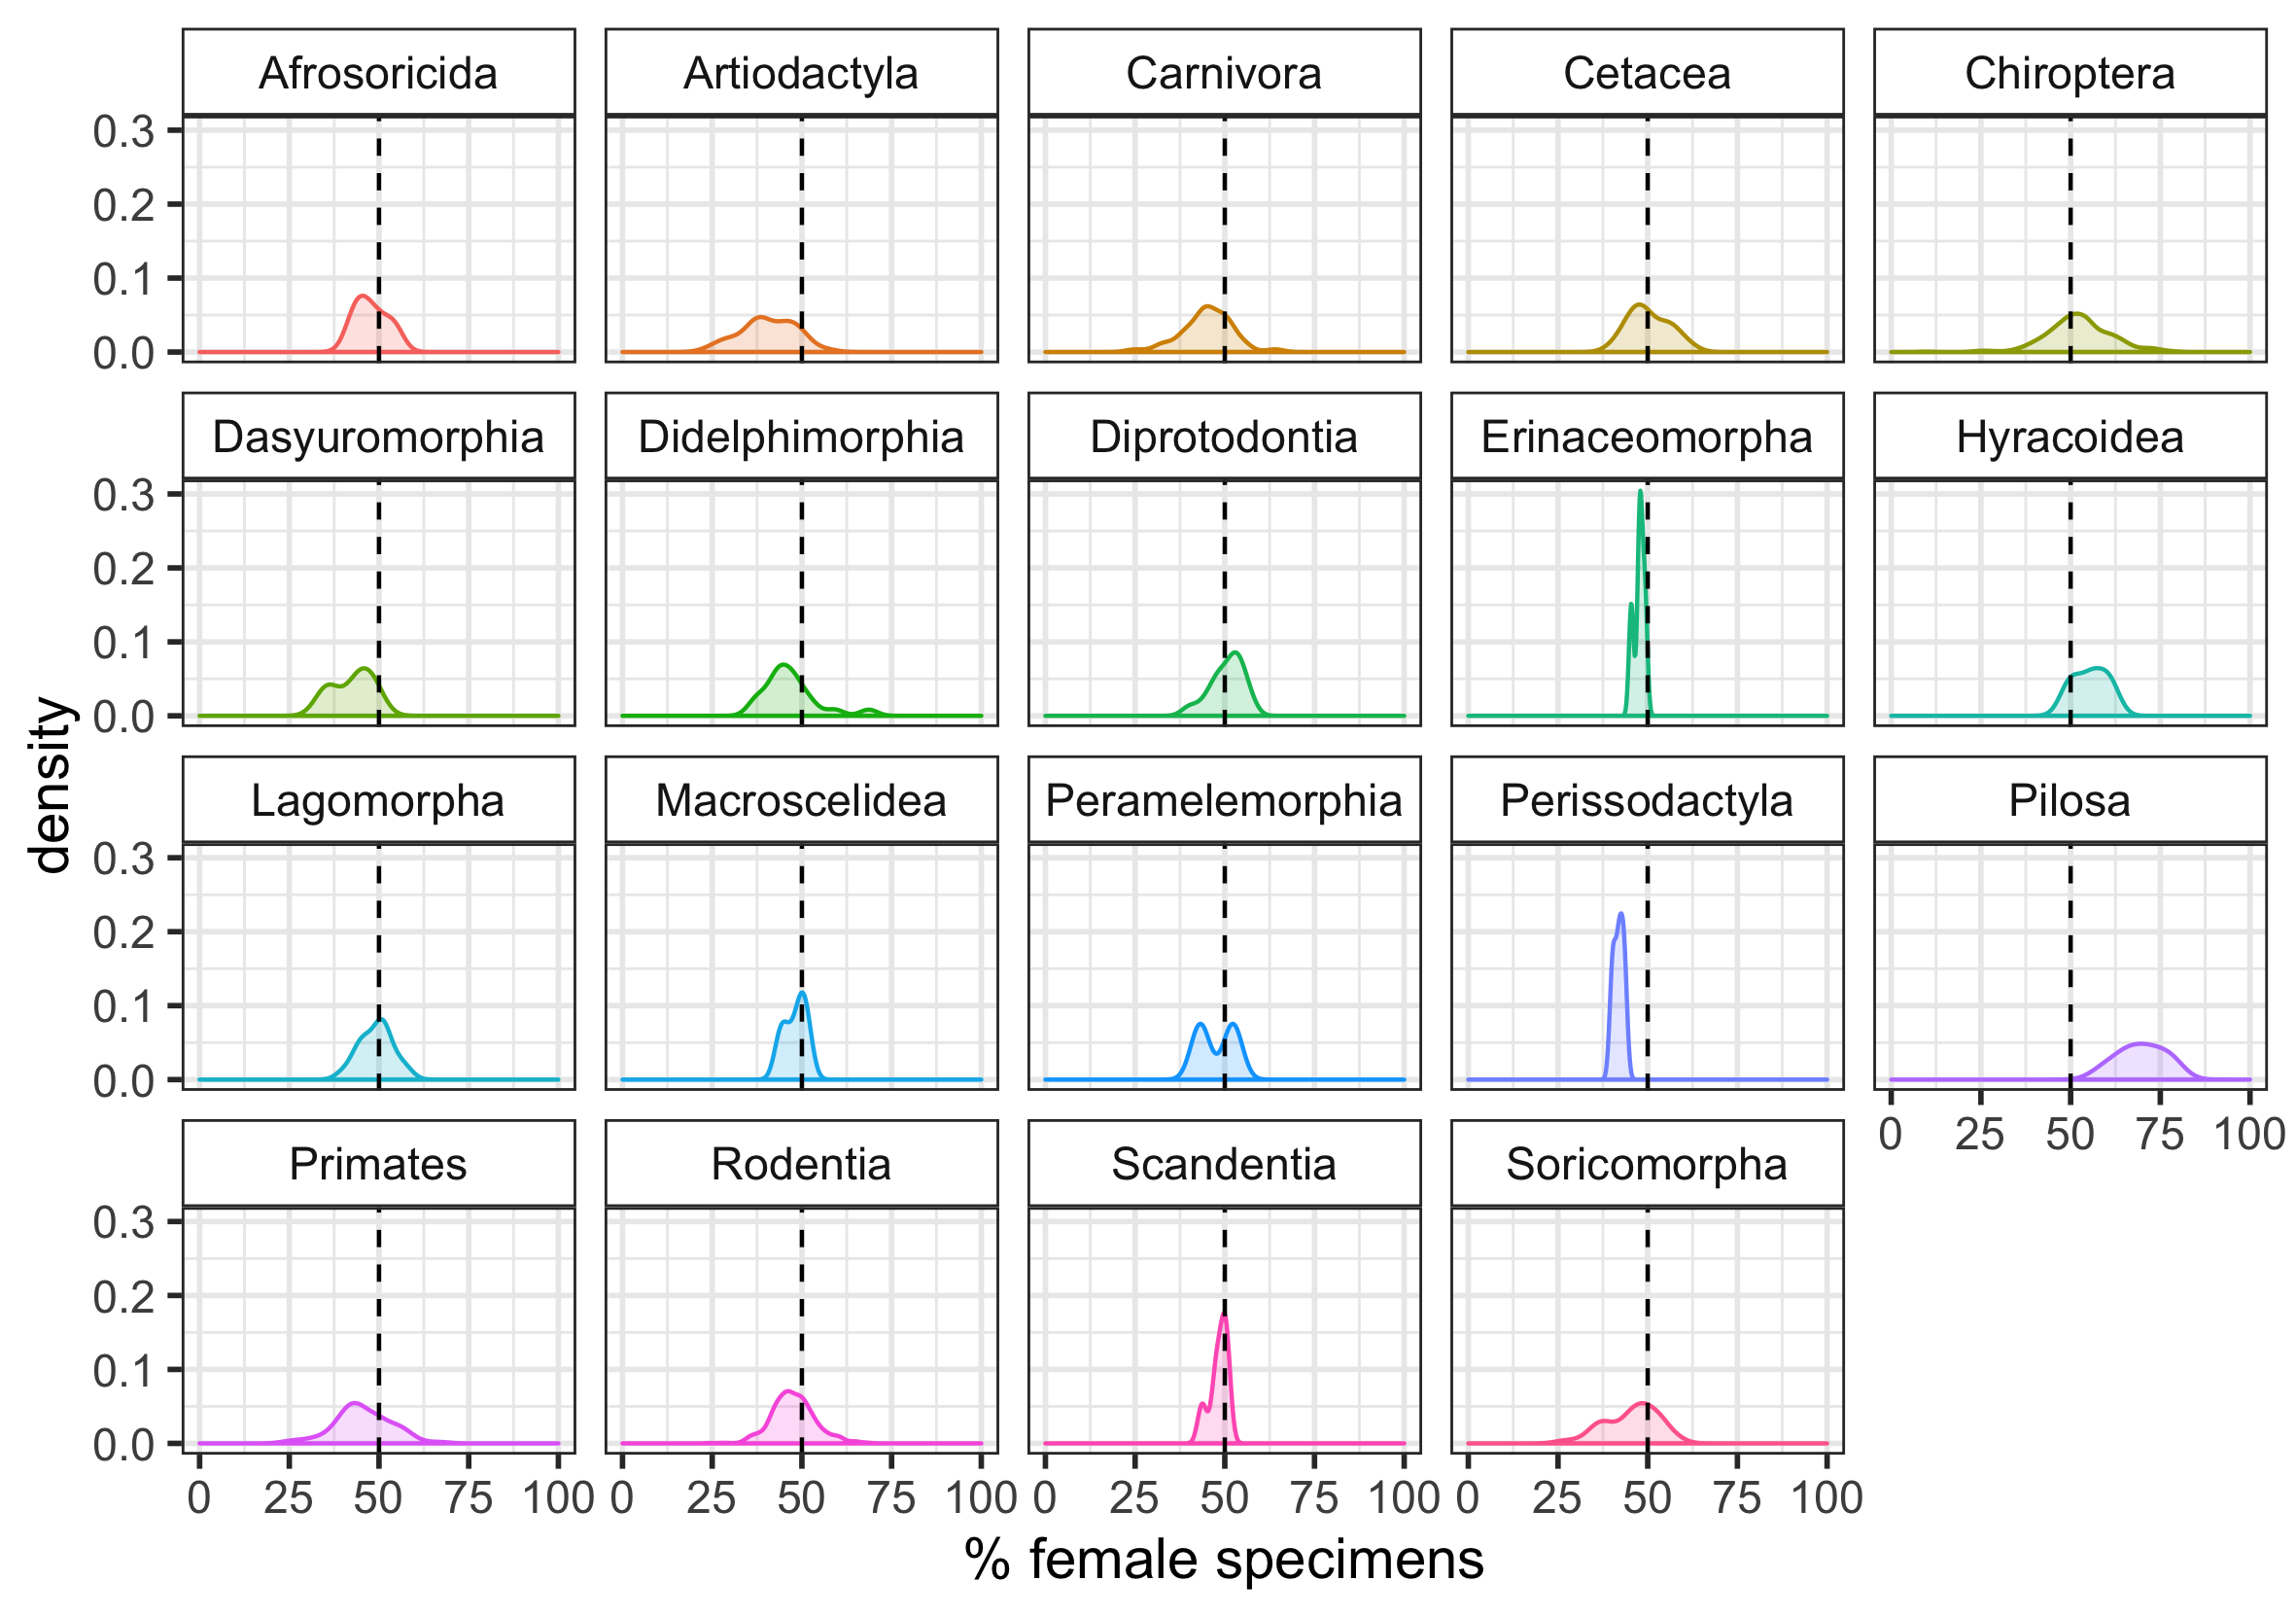
\includegraphics[width = \linewidth]{figures/orders-density-mammals-all.png}
  \caption{Kernel density plots showing the \% female specimens in each species across orders of mammals with at least three species in the dataset. 
  Only species with at least 100 specimens are included. 
  The dashed line represents 50\% female specimens.}
  \label{fig-mammal-orders}
\end{figure}

% figure A6
\begin{figure}
 \centering
  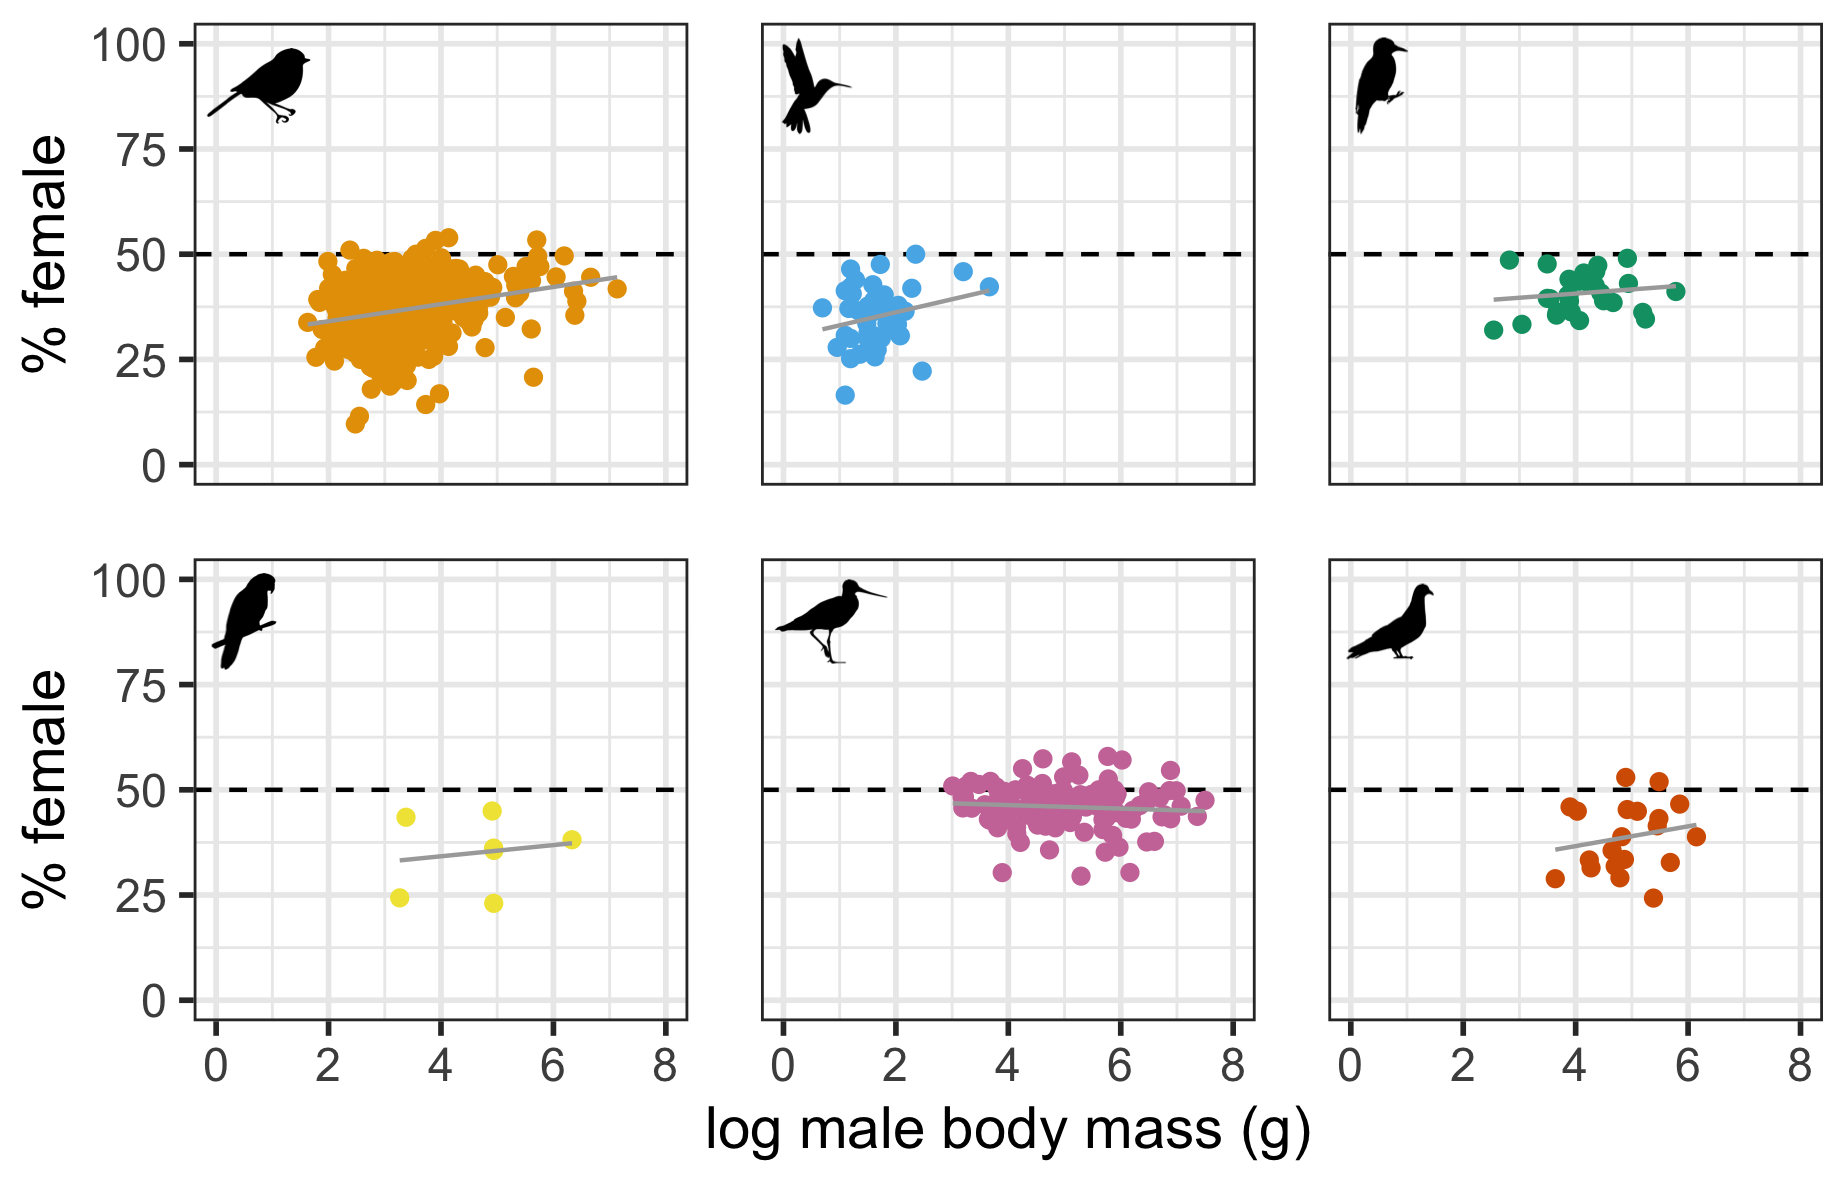
\includegraphics[width = \linewidth]{figures/mass-orders-birds.png}
  \caption{Plots showing how \% female specimens in each species varies with male body mass (g) across the six largest orders of birds (from left to right, top to bottom: Passeriformes, Apodiformes, Piciformes, Psittaciformes, Charadriiformes, and Columbiformes). 
  Only species with at least 100 specimens are included. 
  The dashed line represents 50\% female specimens; grey lines show relationship between the variables using a simple linear regression and are for reference only. 
  Silhouettes are from PhyloPic.org contributed by Ferran Sayol (parrot, hummingbird, tit), Steven Traver (woodpecker) and Alexandre Vong (shorebird).}
  \label{fig-bird-male-mass}
\end{figure}

% figure A7
\begin{figure}
 \centering
  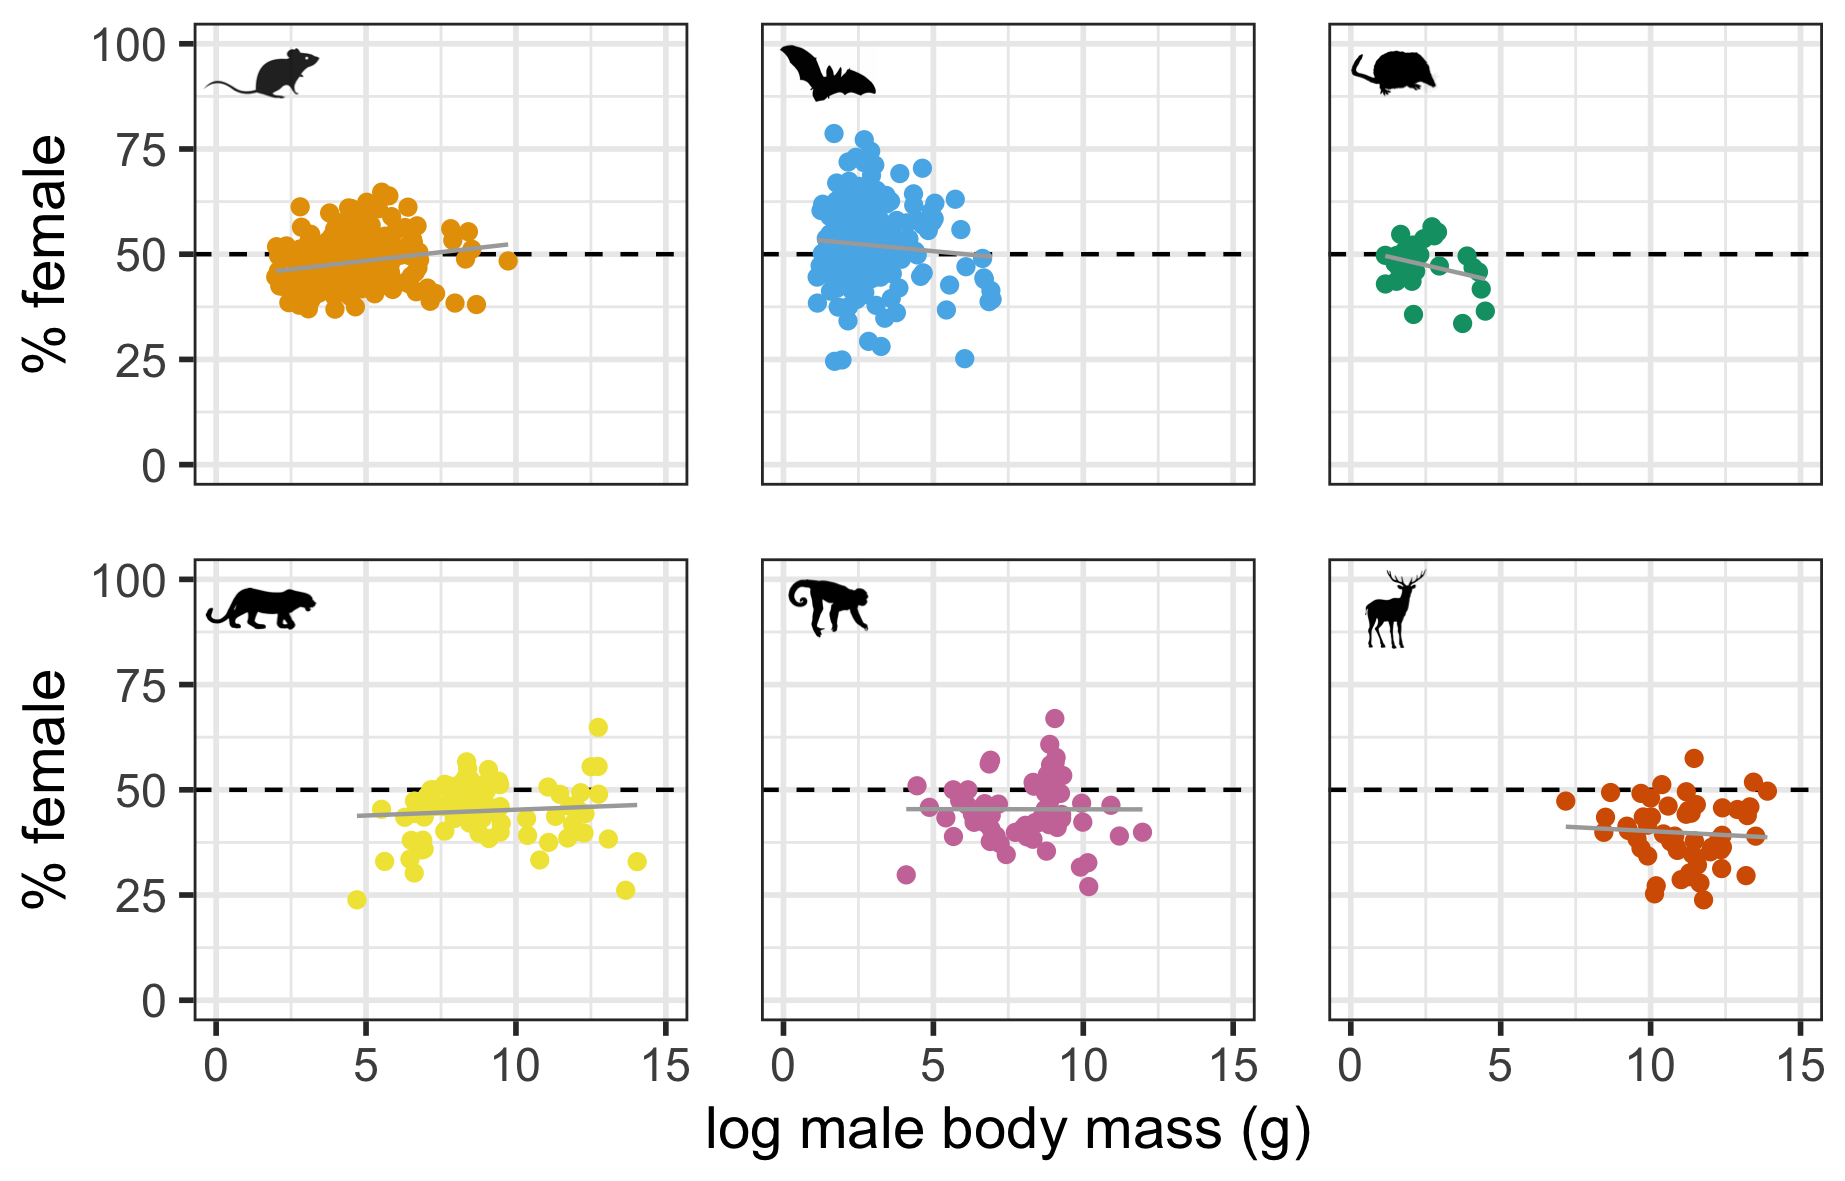
\includegraphics[width = \linewidth]{figures/mass-orders-mammals.png}
  \caption{Plots showing how \% female specimens in each species varies with male body mass (g) across the six largest orders of mammals (from left to right, top to bottom: Rodentia, Chiroptera, Soricomorpha, Carnivora, Primates, and Artiodactyla). 
  Only species with at least 100 specimens are included. 
  The dashed line represents 50\% female specimens; grey lines show relationship between the variables using a simple linear regression and are for reference only. 
  Silhouettes are from PhyloPic.org contributed by Daniel Jaron (mouse), Yan Wong (bat), Becky Barnes (shrew), Lukasiniho (tiger), Sarah Werning (monkey), and Oscar Sanisidro (deer).}
  \label{fig-mammal-male-mass}
\end{figure}

% figure A8
\begin{figure}
 \centering
  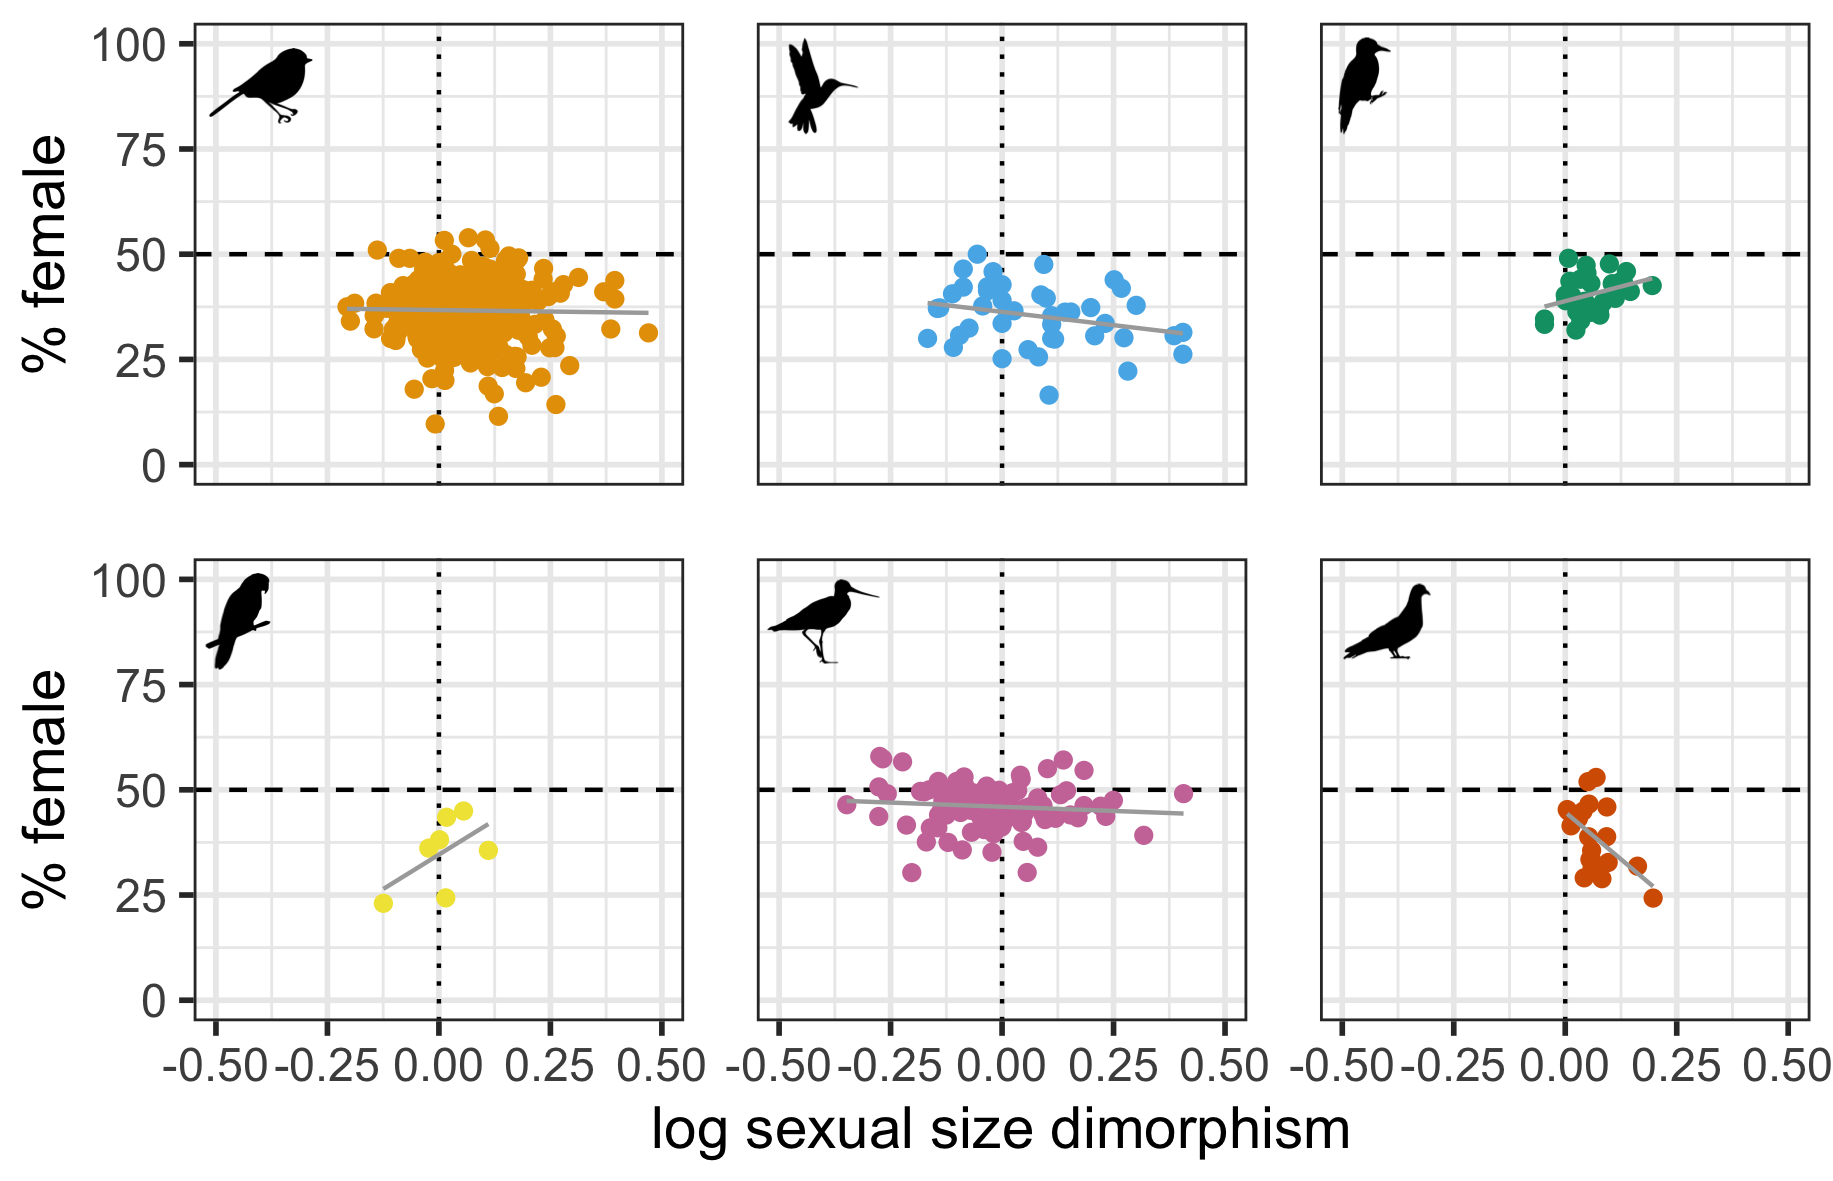
\includegraphics[width = \linewidth]{figures/ssd-orders-birds.png}
  \caption{Plots showing how \% female specimens in each species varies with sexual size dimorphism across the six largest orders of birds (from left to right, top to bottom: Passeriformes, Apodiformes, Piciformes, Psittaciformes, Charadriiformes, and Columbiformes).
  Sexual size dimorphism is male mass divided by female mass. 
  Only species with at least 100 specimens are included. 
  The dashed line represents 50\% female specimens; the dotted line is the point at which males and females have the same body size; grey lines show relationship between the variables using a simple linear regression and are for reference only. 
  Silhouettes are from PhyloPic.org contributed by Ferran Sayol (parrot, hummingbird, tit), Steven Traver (woodpecker) and Alexandre Vong (shorebird).}
  \label{fig-bird-ssd}
\end{figure}

% figure A9
\begin{figure}
 \centering
  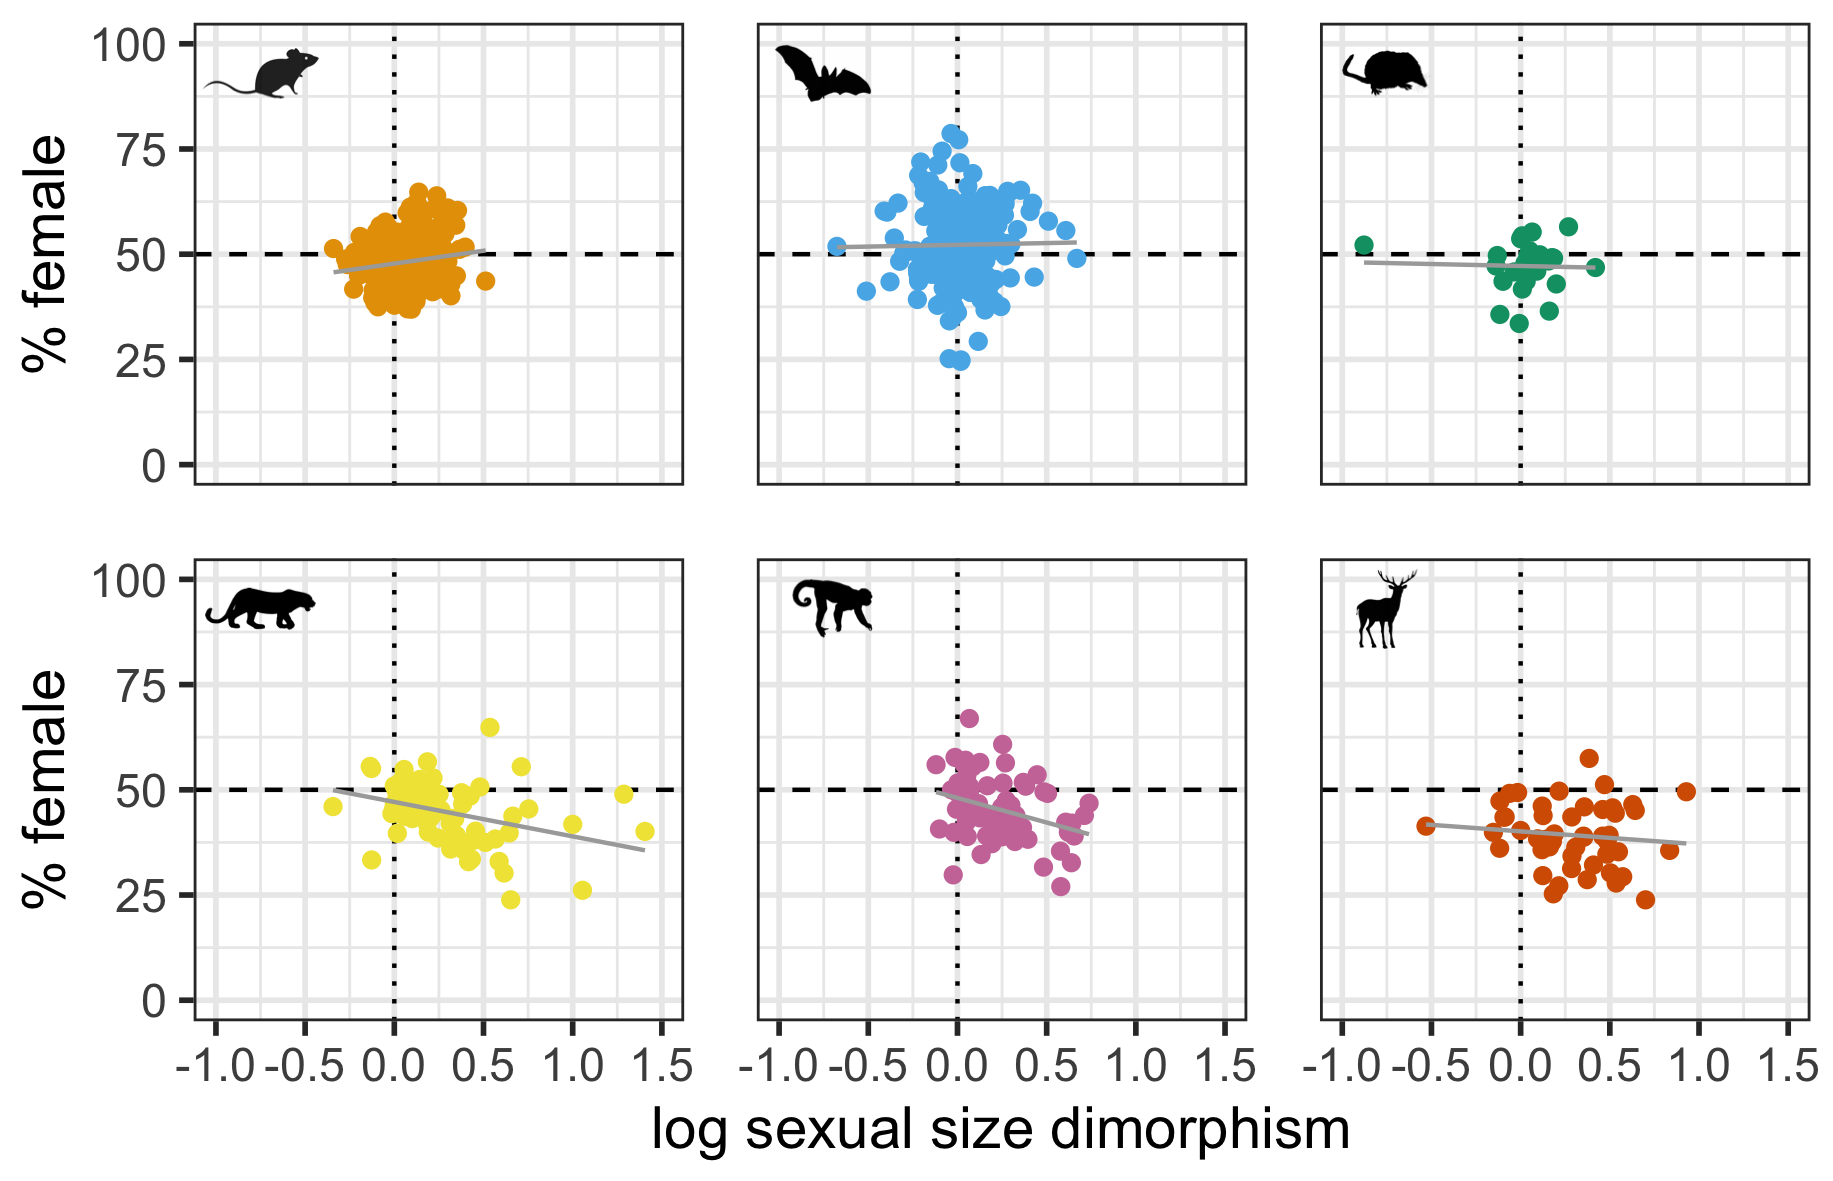
\includegraphics[width = \linewidth]{figures/ssd-orders-mammals.png}
  \caption{Plots showing how \% female specimens in each species varies with sexual size dimorphism across the six largest orders of mammals (from left to right, top to bottom: Rodentia, Chiroptera, Soricomorpha, Carnivora, Primates, and Artiodactyla). 
  Sexual size dimorphism is male mass divided by female mass. 
  Only species with at least 100 specimens are included. 
  The dashed line represents 50\% female specimens; the dotted line is the point at which males and females have the same body size; grey lines show relationship between the variables using a simple linear regression and are for reference only. 
  Silhouettes are from PhyloPic.org contributed by Daniel Jaron (mouse), Yan Wong (bat), Becky Barnes (shrew), Lukasiniho (tiger), Sarah Werning (monkey), and Oscar Sanisidro (deer).}
  \label{fig-mammal-ssd}
\end{figure}


%-------------------------------------------------------------------------------
% Tables
%-------------------------------------------------------------------------------

\newpage
\section*{Supplementary Tables}

% Table A1
% latex table generated in R 3.5.2 by xtable 1.8-3 package
% Thu Apr  4 15:29:25 2019
\begin{longtable}{ll>{\itshape}lcc}
\caption{Species of birds and mammals with the most extreme sex ratios
                  in our data, i.e. species with fewer than 25\% female or fewer 
                  than 25\% male specimens, for species with at least 100 specimens
                  in total. Species with  fewer than 25\% male specimens are highlighted 
                  in bold.} \\ 
  \hline
\textbf{class} & \textbf{order} & \textbf{binomial} & \textbf{n specimens} & \textbf{\% female} \\ 
  \hline
Birds & Passeriformes & Pardalotus striatus & 300 & 9.67 \\ 
  Birds & Passeriformes & Ficedula hypoleuca & 148 & 11.49 \\ 
  Birds & Passeriformes & Camaroptera brachyura & 195 & 11.79 \\ 
  Birds & Columbiformes & Streptopelia tranquebarica & 109 & 13.76 \\ 
  Birds & Passeriformes & Euplectes progne & 112 & 14.29 \\ 
  Birds & Passeriformes & Cinnyris asiaticus & 112 & 14.29 \\ 
  Birds & Passeriformes & Cinnyris mariquensis & 253 & 16.21 \\ 
  Birds & Apodiformes & Chlorostilbon mellisugus & 109 & 16.51 \\ 
  Birds & Passeriformes & Saxicola rubicola & 156 & 16.67 \\ 
  Birds & Passeriformes & Cicinnurus regius & 202 & 16.83 \\ 
  Birds & Passeriformes & Aethopyga siparaja & 321 & 17.76 \\ 
  Birds & Passeriformes & Vireo plumbeus & 106 & 17.92 \\ 
  Birds & Passeriformes & Euplectes macroura & 134 & 18.66 \\ 
  Birds & Passeriformes & Cinnyris mediocris & 127 & 18.90 \\ 
  Birds & Passeriformes & Euplectes albonotatus & 221 & 19.46 \\ 
  Birds & Passeriformes & Aethopyga shelleyi & 122 & 19.67 \\ 
  Birds & Passeriformes & Aethopyga nipalensis & 101 & 19.80 \\ 
  Birds & Passeriformes & Emberiza citrinella & 390 & 20.00 \\ 
  Birds & Passeriformes & Junco hyemalis & 1959 & 20.42 \\ 
  Birds & Passeriformes & Rupicola peruvianus & 130 & 20.77 \\ 
  Birds & Passeriformes & Acrocephalus atyphus & 158 & 21.52 \\ 
  Birds & Passeriformes & Cinnyris chloropygius & 218 & 21.56 \\ 
  Birds & Passeriformes & Cyanocompsa parellina & 111 & 21.62 \\ 
  Birds & Passeriformes & Paradisaea minor & 174 & 21.84 \\ 
  Birds & Passeriformes & Cinnyris venustus & 387 & 21.96 \\ 
  Birds & Apodiformes & Campylopterus hemileucurus & 144 & 22.22 \\ 
  Birds & Passeriformes & Emberiza cirlus & 152 & 22.37 \\ 
  Birds & Passeriformes & Chalcomitra senegalensis & 536 & 22.57 \\ 
  Birds & Passeriformes & Cinnyris chalybeus & 181 & 22.65 \\ 
  Birds & Passeriformes & Oenanthe hispanica & 175 & 22.86 \\ 
  Birds & Passeriformes & Cinnyris pulchellus & 139 & 23.02 \\ 
  Birds & Psittaciformes & Psittacula krameri & 152 & 23.03 \\ 
  Birds & Passeriformes & Myzomela cardinalis & 581 & 23.06 \\ 
  Birds & Passeriformes & Euplectes ardens & 299 & 23.08 \\ 
  Birds & Passeriformes & Aethopyga gouldiae & 117 & 23.08 \\ 
  Birds & Passeriformes & Cyanerpes lucidus & 129 & 23.26 \\ 
  Birds & Passeriformes & Nectarinia famosa & 176 & 23.30 \\ 
  Birds & Passeriformes & Cinnyris habessinicus & 120 & 23.33 \\ 
  Birds & Passeriformes & Lichmera incana & 119 & 23.53 \\ 
  Birds & Passeriformes & Euplectes axillaris & 119 & 23.53 \\ 
  Birds & Passeriformes & Troglodytes musculus & 144 & 23.61 \\ 
  Birds & Apodiformes & Phaethornis longirostris & 192 & 23.96 \\ 
  Birds & Passeriformes & Prunella modularis & 174 & 24.14 \\ 
  Birds & Passeriformes & Piranga olivacea & 505 & 24.16 \\ 
  Birds & Passeriformes & Sporophila minuta & 132 & 24.24 \\ 
  Birds & Columbiformes & Treron calvus & 103 & 24.27 \\ 
  Birds & Psittaciformes & Forpus passerinus & 111 & 24.32 \\ 
  Birds & Passeriformes & Setophaga dominica & 704 & 24.43 \\ 
  Birds & Passeriformes & Malurus lamberti & 126 & 24.60 \\ 
  Birds & Passeriformes & Aimophila rufescens & 142 & 24.65 \\ 
  Birds & Passeriformes & Nectarinia johnstoni & 101 & 24.75 \\ 
  Mammals & Chiroptera & Nyctiellus lepidus & 111 & 9.91 \\ 
  Mammals & Artiodactyla & Ovis ammon & 109 & 23.85 \\ 
  Mammals & Carnivora & Mustela nivalis & 570 & 23.86 \\ 
  Mammals & Rodentia & Allactaga sibirica & 252 & 24.21 \\ 
  Mammals & Chiroptera & Emballonura raffrayana & 167 & 24.55 \\ 
  Mammals & Primates & Homo sapiens & 138 & 24.64 \\ 
  Mammals & Chiroptera & Pteronotus personatus & 410 & 24.88 \\ 
  Mammals & Pilosa & Tamandua tetradactyla & 261 & \textbf{76.63} \\ 
  Mammals & Chiroptera & Chaerephon major & 193 & \textbf{77.20} \\ 
  Mammals & Pilosa & Tamandua mexicana & 157 & \textbf{78.34} \\ 
  Mammals & Chiroptera & Myotis oxyotus & 136 & \textbf{78.68} \\ 
\hline
\label{table-percents}
\end{longtable}


\newpage
% Table A2
% latex table generated in R 3.5.2 by xtable 1.8-3 package
% Thu Apr  4 15:42:54 2019
\begin{longtable}{llccc}
\caption{Median percentages of female specimens within species with at least 
                   100 specimens, or each order of birds and mammals. 
                   Orders with median percentages of female specimens of over 50\% are in bold.} \\ 
  \hline
\textbf{class} & \textbf{order} & \textbf{n species} & \textbf{n specimens} & \textbf{\% female} \\ 
  \hline
Birds & Accipitriformes &  37 & 9738 & 48.76 \\ 
  Birds & Anseriformes &  45 & 12301 & 42.48 \\ 
  Birds & Apodiformes &  64 & 10914 & 37.18 \\ 
  Birds & Bucerotiformes &   5 & 919 & 40.70 \\ 
  Birds & Caprimulgiformes &  24 & 5565 & 44.19 \\ 
  Birds & Charadriiformes & 148 & 43393 & 46.32 \\ 
  Birds & Coliiformes &   2 & 491 & 37.92 \\ 
  Birds & Columbiformes &  46 & 8464 & 36.77 \\ 
  Birds & Coraciiformes &  27 & 7377 & 44.71 \\ 
  Birds & Cuculiformes &  29 & 6223 & 41.32 \\ 
  Birds & Falconiformes &  14 & 5577 & 47.70 \\ 
  Birds & Galliformes &  37 & 13062 & 40.99 \\ 
  Birds & Gaviiformes &   3 & 585 & 49.03 \\ 
  Birds & Gruiformes &  20 & 5082 & 45.22 \\ 
  Birds & Passeriformes & 1021 & 317414 & 38.39 \\ 
  Birds & Pelecaniformes &  26 & 6355 & 44.81 \\ 
  Birds & Phaethontiformes &   2 & 684 & 47.88 \\ 
  Birds & Piciformes &  74 & 19003 & 43.27 \\ 
  Birds & Podicipediformes &   9 & 1746 & 45.41 \\ 
  Birds & Procellariiformes &  33 & 6842 & 47.90 \\ 
  Birds & Psittaciformes &  33 & 5011 & 40.57 \\ 
  Birds & Strigiformes &  24 & 6570 & 47.33 \\ 
  Birds & Suliformes &  12 & 2929 & 47.19 \\ 
  Birds & Tinamiformes &   4 & 608 & \textbf{50.36} \\ 
  Birds & Trogoniformes &   7 & 1070 & 40.50 \\ 
  Mammals & Afrosoricida &   4 & 459 & 47.25 \\ 
  Mammals & Artiodactyla &  60 & 15855 & 39.71 \\ 
  Mammals & Carnivora &  91 & 46610 & 45.37 \\ 
  Mammals & Cetacea &  16 & 8929 & 49.30 \\ 
  Mammals & Chiroptera & 366 & 195777 & \textbf{52.19} \\ 
  Mammals & Cingulata &   2 & 613 & 37.15 \\ 
  Mammals & Dasyuromorphia &   3 & 436 & 43.75 \\ 
  Mammals & Dermoptera &   1 & 103 & \textbf{55.34} \\ 
  Mammals & Didelphimorphia &  20 & 9240 & 45.40 \\ 
  Mammals & Diprotodontia &  15 & 3303 & \textbf{52.33} \\ 
  Mammals & Erinaceomorpha &   4 & 1176 & 47.88 \\ 
  Mammals & Hyracoidea &   3 & 831 & \textbf{55.70} \\ 
  Mammals & Lagomorpha &  25 & 12127 & \textbf{50.22} \\ 
  Mammals & Macroscelidea &   9 & 2412 & 48.93 \\ 
  Mammals & Monotremata &   1 & 106 & 40.57 \\ 
  Mammals & Paucituberculata &   2 & 484 & 39.84 \\ 
  Mammals & Peramelemorphia &   2 & 465 & 47.71 \\ 
  Mammals & Perissodactyla &   3 & 498 & 42.00 \\ 
  Mammals & Pholidota &   1 & 126 & \textbf{51.59} \\ 
  Mammals & Pilosa &   7 & 1293 & \textbf{71.07} \\ 
  Mammals & Primates &  80 & 19856 & 44.79 \\ 
  Mammals & Rodentia & 701 & 488124 & 47.34 \\ 
  Mammals & Scandentia &   6 & 1929 & 48.95 \\ 
  Mammals & Sirenia &   1 & 152 & 46.71 \\ 
  Mammals & Soricomorpha &  90 & 46618 & 46.78 \\ 
\hline
\label{table-orders}
\end{longtable}


\newpage
% Table A3
% latex table generated in R 3.5.2 by xtable 1.8-3 package
% Thu Apr  4 15:29:25 2019
\begin{longtable}{lcccc}

  \caption{Outputs from generalised linear models (GLMs) with quasibinomial errors where the response variable is the number of male and female specimens for each species, for species with more than 100 specimens. mass = log male body mass (g); SSD = log male body mass/female body mass. Significance testing uses Type II ANOVA. df = degrees of freedom; SE = standard error.} \\ 
  
  \hline
  \multicolumn{5}{c}{\textbf{Birds}} \\
  \hline
  \textbf{coefficients} & \textbf{F} & \textbf{df} & \textbf{p} & \textbf{$slope \pm SE$} \\ 
  \hline

  mass & 273.1 & 1, 849 & \textbf{\textless 0.001} & $0.102 \pm 0.006$ \\
  \hline
  mass & 40.33 & 1, 803 & \textbf{\textless 0.001} & NA \\
  order & 10.06 & 24, 803 & \textbf{\textless 0.001} & \\
  mass:order & 1.183 & 22, 803 & 0.254 & \\
  \hline

  SSD & 41.23 & 1, 827 & \textbf{\textless 0.001} & $-0.436 \pm 0.068$ \\
  \hline
  SSD & 0.317 & 1, 782 & 0.574 & NA \\
  order & 18.92 & 24, 782 & \textbf{\textless 0.001} & \\
  SSD:order & 1.501 & 21, 782 & 0.069 & \\
  \hline

  SSD & 2.269 & 1, 741 & 0.132 & NA \\
  mass & 41.40 & 1, 741 & \textbf{\textless 0.001} &  \\
  order & 6.800 & 24, 741 & \textbf{\textless 0.001} & \\
  SSD:mass & 0.073 & 1, 741 & 0.787 & \\
  SSD:order & 1.070 & 20, 741 & 0.376 & \\
  mass:order & 0.918 & 20, 741 & 0.563 & \\
  SSD:mass:order & 0.989 & 19, 741 & 0.472 & \\

  \hline
  \multicolumn{5}{c}{\textbf{Mammals}} \\
  \hline
  \textbf{coefficients} & \textbf{F} & \textbf{df} & \textbf{p} & \textbf{$slope \pm SE$} \\ 
  \hline

  mass & 46.24 & 1, 785 & \textbf{\textless 0.001} & $-0.025\pm 0.004$ \\
  \hline
  mass & 21.15 & 1, 751 & \textbf{\textless 0.001} & NA \\
  order & 14.13 & 19, 751 & \textbf{\textless 0.001} & \\
  mass:order & 2.802 & 15, 751 & \textbf{\textless 0.001} & \\
  \hline

  SSD & 27.34 & 1, 715 & \textbf{\textless 0.001} & $-0.244 \pm 0.047$ \\
  \hline
  SSD & 0.052 & 1, 681 & 0.819 & NA \\
  order & 13.68 & 19, 681 & \textbf{\textless 0.001} & \\
  SSD:order & 1.339 & 15, 681 & 0.173 & \\
  \hline

  SSD & 0.672 & 1, 660 & 0.413 & NA \\
  mass & 31.31 & 1, 660 & \textbf{\textless 0.001} &  \\
  order & 14.38 & 19, 660 & \textbf{\textless 0.001} & \\
  SSD:mass & 5.247 & 1, 660 & \textbf{0.023} & \\
  SSD:order & 1.979 & 10, 660 & \textbf{0.033} & \\
  mass:order & 4.094 & 10, 660 & \textbf{\textless 0.001} & \\
  SSD:mass:order & 0.810 & 9, 660 & 0.607 & \\

\hline
\label{table-outputs}
\end{longtable}


%-------------------------------------------------------------------------------
% Methods
%-------------------------------------------------------------------------------

\newpage
\section*{Supplementary Methods}

We expect large skews in the proportion of male or female specimens when sample size is low, but the ratio of male:female specimens should approach 50:50 as more specimens are added if there is no bias. 
Most species in our dataset were represented by only a few specimens (Figure \ref{fig-histograms}), with large skews in the percentage of female specimens (in both directions) at low numbers (Figure \ref{fig-hex}).

To test whether this may influence our analyses, we used generalised linear models (GLM) with binomial errors, with the proportion of female specimens (success) and the proportion of male specimens (failure) for each species as the response variable, and the log number of specimens per species as the explanatory variable. 
We then used standard model checks for GLMs (Q-Q plot, histogram of residuals, residuals vs. linear predictors, response vs. fitted values) to assess model fit. 
The model showed massive heteroscedasticity in the residuals, due to the skew in proportions when sample size is low. 
We therefore repeated the analysis, removing species with fewer than 20, 50, 100, 150 and 200 specimens in turn. 
The best fitting model, without losing too much data, was a model with species with more than 100 specimens. 
There is still a significant positive relationship between the number of specimens and the proportion of female specimens but this is not unusual with such a large dataset, and the effect size is extremely low ($slope \pm SE = 0.034 \pm 0.001$, $z_3257 = 24.86$, $p < 0.001$) so we exclude this variable from further analyses.

\end{document}